\documentclass[tikz, border=10pt]{standalone}
\usepackage{iftex}
\ifluatex
  \usepackage{fontspec}
  \usepackage{unicode-math}
  \setmainfont{Fira Sans}
  \setmonofont{Fira Mono}
  \setmathfont{Fira Math}
  \setmathfont{STIX Two Math}[range={"29F5,"2216}]
\else
  \usepackage[T1]{fontenc}
\fi

\usepackage{amsmath}
\usepackage{tikz}
\usetikzlibrary{arrows.meta}
\tikzset{every node/.style={font=\Large}}

% Theme toggle: \darkbgfalse for light background preview.
\newif\ifdarkbg
\darkbgtrue
\ifdarkbg
  \colorlet{axiscol}{white}
  \colorlet{gridcol}{white!30!black}
  \colorlet{ticklabelcol}{white}
  \colorlet{funcol}{lime!90!green}
  \colorlet{auxcol}{white!55!black}
\else
  \colorlet{axiscol}{black}
  \colorlet{gridcol}{black!25!white}
  \colorlet{ticklabelcol}{black}
  \colorlet{funcol}{blue!70!black}
  \colorlet{auxcol}{black!40!white}
\fi

% x: -6 to 1   (7 units)    xscale=1.00 → ~7.0 cm wide
% y: -21 to 9  (30 units)   yscale=0.28 → ~8.4 cm tall
% Roots: (-5,0) and (0,0). Vertex: (-2.5, -18.75).
\begin{document}
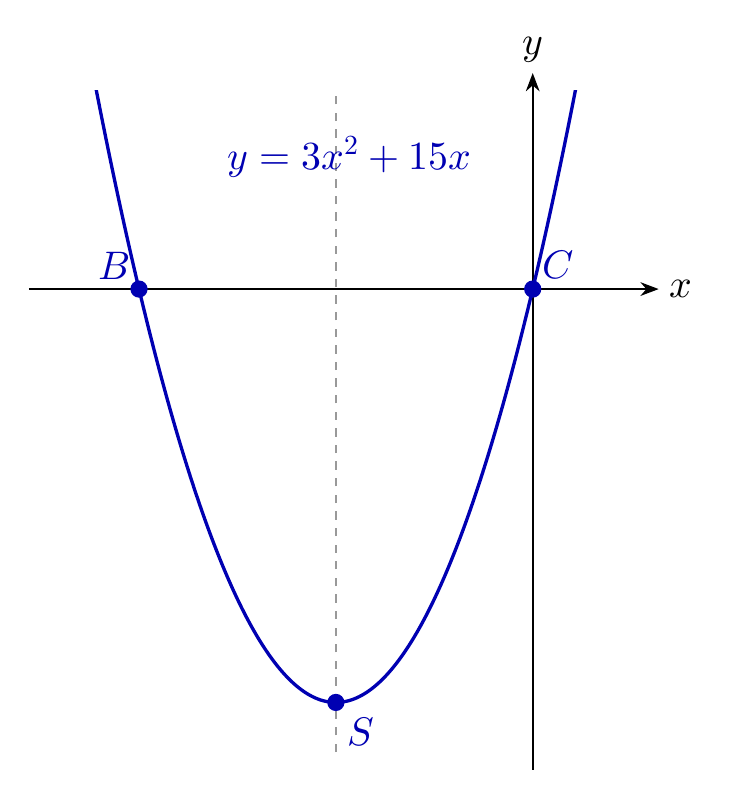
\begin{tikzpicture}[xscale=1.00, yscale=0.28, >=Stealth]

  % Cartesian grid.
  % \draw[step=1, very thin, gridcol] (-6,-21) grid (1,9);

  % Axes.
  \draw[->, thick, axiscol] (-6.4,0) -- (1.6,0)
    node[right, text=axiscol] {$x$};
  \draw[->, thick, axiscol] (0,-21.8) -- (0,9.8)
    node[above, text=axiscol] {$y$};

  % Tick marks — x axis (skip 0, occupied by point C).
  % \foreach \x in {-6,-5,-4,-3,-2,-1,1} {
  %   \draw[axiscol] (\x, 3pt) -- (\x, -3pt)
  %     node[below, text=ticklabelcol] {$\x$};
  % }

  % Tick marks — y axis (major every 6, minor every 3).
  % \foreach \y in {-18,-12,-6,6} {
  %   \draw[axiscol] (3pt,\y) -- (-3pt,\y)
  %     node[left, text=ticklabelcol] {$\y$};
  % }
  % \foreach \y in {-21,-15,-9,-3,3,9} {
  %   \draw[axiscol] (2pt,\y) -- (-2pt,\y);
  % }

  % Function curve: y = 3x^2 + 15x, clipped to the window.
  \begin{scope}
    \clip (-6,-21) rectangle (1,9);
    \draw[domain=-6:1, smooth, very thick, funcol, samples=120]
      plot (\x, {3*(\x)^2 + 15*(\x)});
  \end{scope}

  % Axis of symmetry.
  \draw[dashed, thick, auxcol] (-2.5,-21) -- (-2.5,9);

  % Equation label in an empty area left of the vertex.
  \node[right, text=funcol] at (-4.0,6.0) {$y=3x^2+15x$};

  % X-axis intersections.
  \node[circle, fill=funcol, inner sep=2.2pt] at (-5,0) {};
  \node[above left, text=funcol] at (-5,0) {$B$};

  \node[circle, fill=funcol, inner sep=2.2pt] at (0,0) {};
  \node[above right, text=funcol] at (0,0) {$C$};

  \node[circle, fill=funcol, inner sep=2.2pt] at (-2.5,-18.75) {};
  \node[below, text=funcol] at (-2.2,-19.0) {$S$};

\end{tikzpicture}
\end{document}
